\section{Question 3}

Given the following recurrent neural network diagram, answer the questions below. Note that for simplicity, all values (inputs, weights, and outputs) are scalar values. Also, assume that all activation functions are sigmoid functions.

\begin{figure}[H]
    \centering
    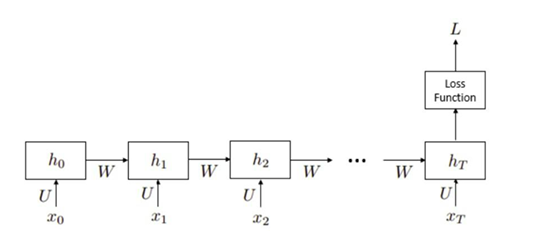
\includegraphics[width=0.6\textwidth]{Q3.png}
    \caption{Network Architecture}
\end{figure}

\subsection{part A} 
Write the gradient of \( h_t \) with respect to \( h_{t+1} \), i.e., \( \frac{\partial L}{\partial h_t} \) in terms of \( \frac{\partial L}{\partial h_{t+1}} \) (\( 1 \leq t \leq T-1 \)).
\begin{qsolve}
  \begin{qsolve}[]
based on the Architecture we have:
\[
h_t = \sigma(U x_t + W h_{t-1}),
\]

To calculate \( \frac{\partial L}{\partial h_t} \), the chain rule gives:

\[
\frac{\partial L}{\partial h_t} = \frac{\partial L}{\partial h_{t+1}} \cdot \frac{\partial h_{t+1}}{\partial h_t}.
\]

Using the recurrence relation for \( h_{t+1} \):

\[
h_{t+1} = \sigma(U x_{t+1} + W h_t),
\]

the derivative of \( h_{t+1} \) with respect to \( h_t \) is:

\[
\frac{\partial h_{t+1}}{\partial h_t} = \sigma'(U x_{t+1} + W h_t) \cdot W,
\]

where \( \sigma'(z) = \sigma(z) (1 - \sigma(z)) \) is the derivative of the sigmoid function.

Substituting this back, we get:

\[
\frac{\partial L}{\partial h_t} = \frac{\partial L}{\partial h_{t+1}} \cdot \sigma'(U x_{t+1} + W h_t) \cdot W.
\]

so the final answer is:

\[
\frac{\partial L}{\partial h_t} = \frac{\partial L}{\partial h_{t+1}} \cdot \sigma(U x_{t+1} + W h_t) \cdot (1 - \sigma(U x_{t+1} + W h_t)) \cdot W.
\]
  \end{qsolve}
\end{qsolve}
\subsection{part B}
Using the relationship from part (a), write the gradient \( h_t \) in a chain-like form with respect to the gradient \( h_T \).

\begin{qsolve}
  \begin{qsolve}[]
    From part (a), we know the relationship for the gradient of \( L \) with respect to \( h_t \) in terms of \( \frac{\partial L}{\partial h_{t+1}} \) is given by:

    \[
    \frac{\partial L}{\partial h_t} = \frac{\partial L}{\partial h_{t+1}} \cdot W \cdot \sigma'(U x_{t+1} + W h_t).
    \]
    
    To express \( \frac{\partial L}{\partial h_t} \) in terms of \( \frac{\partial L}{\partial h_T} \), we use the recursive nature of this relationship:
    
    \[
    \frac{\partial L}{\partial h_t} = \frac{\partial L}{\partial h_T} \cdot \prod_{k=t+1}^T \left(W \cdot \sigma'(U x_k + W h_{k-1})\right).
    \]
    
    This equation indicates that the gradient \( \frac{\partial L}{\partial h_t} \) depends on the gradient at the final time step \( \frac{\partial L}{\partial h_T} \) and accumulates a product of weights \( W \) and the sigmoid derivatives \( \sigma'(U x_k + W h_{k-1}) \) for all subsequent time steps from \( t+1 \) to \( T \).
    
    Thus, the chain-like form of the gradient is:
    
    \[
    \frac{\partial L}{\partial h_t} = \frac{\partial L}{\partial h_T} \cdot \prod_{k=t+1}^T \left(W \cdot \sigma'(U x_k + W h_{k-1})\right),
    \]
  \end{qsolve}
\end{qsolve}
\subsection{part C}
One important method for preventing the vanishing and exploding gradients is to initialize the network weights correctly. Describe how to set the maximum value of \( W \) such that the gradients neither vanish nor explode. (Hint: Find the upper bound for the gradient \( h_t \).)
\begin{qsolve}
  \begin{qsolve}[]

    To determine the upper bound on \( W \), we use the expression for the gradient \( \frac{\partial L}{\partial h_t} \) derived earlier:

    \[
    \frac{\partial L}{\partial h_t} = \frac{\partial L}{\partial h_T} \cdot \prod_{k=t+1}^T \left(W \cdot \sigma'(U x_k + W h_{k-1})\right).
    \]
    
    The derivative of the sigmoid function, \( \sigma'(z) = \sigma(z)(1 - \sigma(z)) \), achieves its maximum value at \( \frac{1}{4} \). Therefore, for any \( k \), we have:
    
    \[
    \sigma'(U x_k + W h_{k-1}) \leq \frac{1}{4}.
    \]
    
    Substituting this upper bound into the gradient expression, the magnitude of \( \frac{\partial L}{\partial h_t} \) can be bounded as:
    \splitqsolve[\splitqsolve]    
    \[
    \left| \frac{\partial L}{\partial h_t} \right| \leq \left| \frac{\partial L}{\partial h_T} \right| \cdot \prod_{k=t+1}^T \left| W \right| \cdot \frac{1}{4}.
    \]
    
    Simplifying further, we obtain:

    \[
    \left| \frac{\partial L}{\partial h_t} \right| \leq \left| \frac{\partial L}{\partial h_T} \right| \cdot |W|^{T-t} \cdot \left(\frac{1}{4}\right)^{T-t}.
    \]
    
  \end{qsolve}
\end{qsolve}
\subsection{part D}
Another method to prevent the vanishing gradient problem is to use skip-connections. The following diagram shows that at each time step \( t \), \( h_t \) is connected to \( h_{t+2} \) as well as \( h_{t+1} \). Now, rewrite the gradient of \( h_t \) with respect to \( h_{t+2} \) and explain why this approach effectively reduces the vanishing gradient problem (\( 1 \leq t \leq T-2 \)).
\begin{figure}[H]
    \centering
    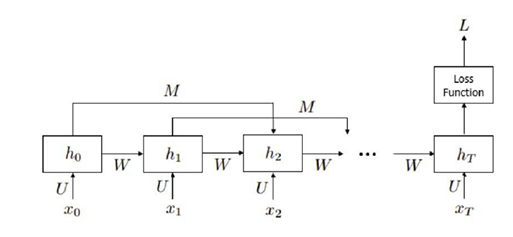
\includegraphics[width=0.7\textwidth]{Q3_2.png}
    \caption{Network Architecture}
\end{figure}
\begin{qsolve}
  \begin{qsolve}[]
  
The gradient of the loss \( L \) with respect to \( h_t \) can be expressed using the chain rule, considering both the direct contribution from \( h_{t+2} \) and the indirect contribution through \( h_{t+1} \). This is written as:

\[
\frac{\partial L}{\partial h_t} = \frac{\partial L}{\partial h_{t+2}} \cdot \frac{\partial h_{t+2}}{\partial h_t} + \frac{\partial L}{\partial h_{t+1}} \cdot \frac{\partial h_{t+1}}{\partial h_t}.
\]

The skip-connection introduces a direct path from \( h_t \) to \( h_{t+2} \), which contributes to \( \frac{\partial h_{t+2}}{\partial h_t} \). This term can be expressed as:
\[
\frac{\partial h_{t+2}}{\partial h_t} = \sigma'(W h_{t+1} + M h_t + U x_{t+2}) \cdot M + \sigma'(W h_{t+1} + M h_t + U x_{t+2}) \cdot W \cdot \frac{\partial h_{t+1}}{\partial h_t}.
\]

Substituting the gradient \( \frac{\partial h_{t+1}}{\partial h_t} \), which is:
\splitqsolve[\splitqsolve]
\[
\frac{\partial h_{t+1}}{\partial h_t} = \sigma'(W h_t + M h_{t-1} + U x_{t+1}) \cdot W,
\]

we get:

\[
\frac{\partial h_{t+2}}{\partial h_t} = \sigma'(W h_{t+1} +
\]
\[ 
M h_t + U x_{t+2}) \cdot M + \sigma'(W h_{t+1} + M h_t + U x_{t+2}) \cdot W \cdot \sigma'(W h_t + M h_{t-1} + U x_{t+1}) \cdot W.
\]

Finally, substituting this back into the expression for \( \frac{\partial L}{\partial h_t} \), we get:

\[
\frac{\partial L}{\partial h_t} = \frac{\partial L}{\partial h_{t+2}} \cdot ( \sigma'(W h_{t+1} +
M h_t + U x_{t+2}) \cdot M 
\]
\[
+ \sigma'(W h_{t+1} + M h_t + U x_{t+2}) \cdot W \cdot \sigma'(W h_t + M h_{t-1} + U x_{t+1}) \cdot W )
\]

\[
+ \frac{\partial L}{\partial h_{t+1}} \cdot \sigma'(W h_t + M h_{t-1} + U x_{t+1}) \cdot W.
\]

The inclusion of the term \( M \) in the gradient ensures a direct contribution to \( \frac{\partial h_{t+2}}{\partial h_t} \), bypassing the dependence on repeated weight multiplications. This reduces the risk of the gradients vanishing, as the direct path provided by the skip-connection does not involve long chains of activations and weight products. This ensures more stable gradient flow and facilitates training for deeper recurrent networks or longer sequences.

  \end{qsolve}
\end{qsolve}
\subsection{part E}
One of the ways to prevent gradient explosion is gradient clipping. This can be done in two ways: clipping by value and clipping by norm. Explain these two methods separately. Also, explain the advantages of clipping by norm over clipping by value.
\begin{qsolve}
  \begin{qsolve}[]
    Gradient explosion occurs when gradients become too large, making training unstable. Gradient clipping solves this by limiting the size of gradients, either by value or by norm. 

    Clipping by value restricts each gradient component to a fixed range, such as \([-\text{threshold}, \text{threshold}]\). This method is simple but does not consider the overall gradient magnitude or direction.
    
    Clipping by norm adjusts the entire gradient vector if its norm exceeds a threshold. The vector is scaled down to make its norm equal to the threshold, preserving the gradient's direction.
    
    Clipping by norm is generally better because it ensures consistent gradient direction and controls the total gradient size, which is especially useful in large models.      
  \end{qsolve}
\end{qsolve}